\section{Evaluation}\label{sec:results}

%In this section, we will present our evaluation results of the \systemname.
We conducted comprehensive evaluation of \systemname~through laboratory studies involving
human subjects -- our studies were approved by the Institutional Review Board (IRB) of our
institution. In the first phase of evaluation, we collected from volunteer participants accelerometer sensor
readings with Google Glass. We analyzed these traces offline on a PC.
Our evaluations are primarily aimed at determining the accuracy of detecting
and differentiating users based on their head-movements, and understanding
the effect of important parameters such as similarity metric, length of the music cue, training
data-set size and sampling rate. In addition to authentication accuracy, we also evaluated how robust is \systemname~against intentional imitation.
In the second phase of evaluation, We also measured the response time of our Google
Glass implementation of \systemname.

%based on profiling the execution time of each key
%functions associated with \systemname, on the Google Glass device.

\begin{figure}
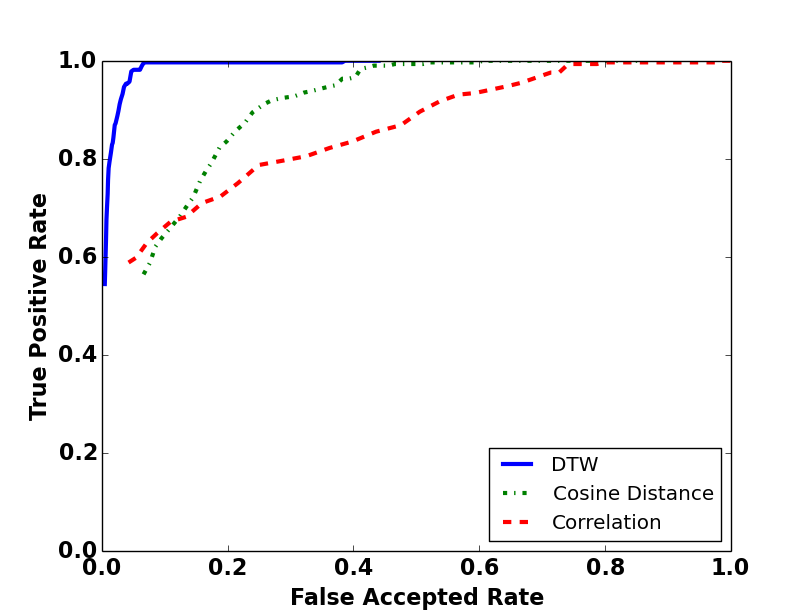
\includegraphics[width=\columnwidth]{figure/roc_dtw_cos_cor.png}
\caption{\label{fig:roc_dtw_cos_cor} The impact of the distance computing algorithm (i.e., DTW, cosine distance, and Correlation). In this set of results, we varied the value of $n$ from 0.0 to 10.0 with an increment of 0.1, resulting in 100 data points in each case. We then plotted the TPR (y-axis) and FAR (x-axis) for each data point. The results show that DTW delivers much better accuracies than the other two distance algorithms. As a result, in the remaining of the study, we will choose DTW for distance computing.}
\end{figure}

\begin{figure}
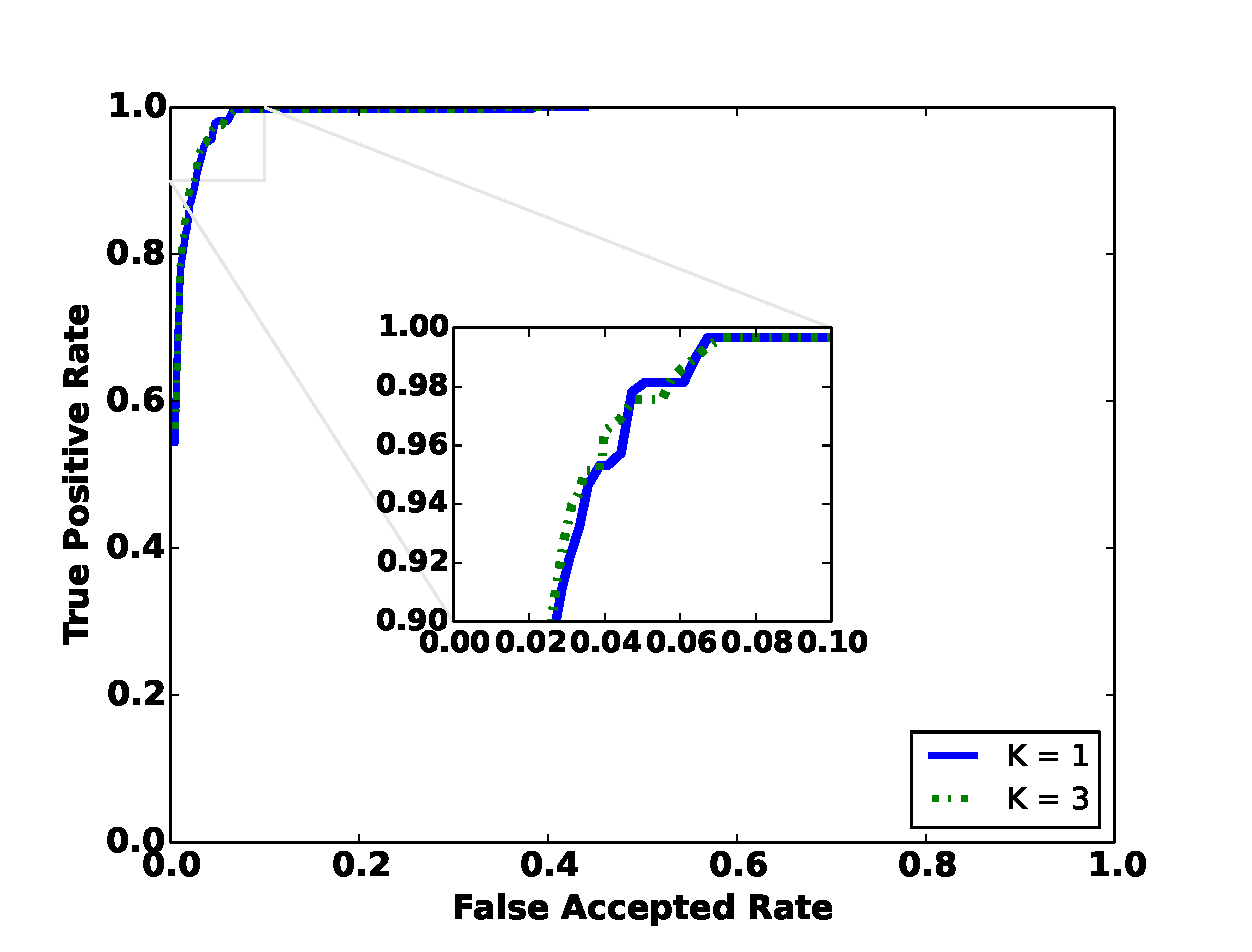
\includegraphics[width=\columnwidth]{figure/roc_k_value.eps}
\caption{\label{fig:roc_k_value} The impact of different K values: $K=1$ and $K=3$. In this set of results, we varied the value of $n$ from 0.0 to 10.0 with an increment of 0.1, resulting in 100 data points in each case. We then plotted the TPR (y-axis) and FAR (x-axis) for each data point. The results show that voting schemes ($K=3$) provide minor improvement on the performance. As a result, in the remaining of the study, we will choose $K=1$.}
\end{figure}



\begin{figure}[t]
\centering
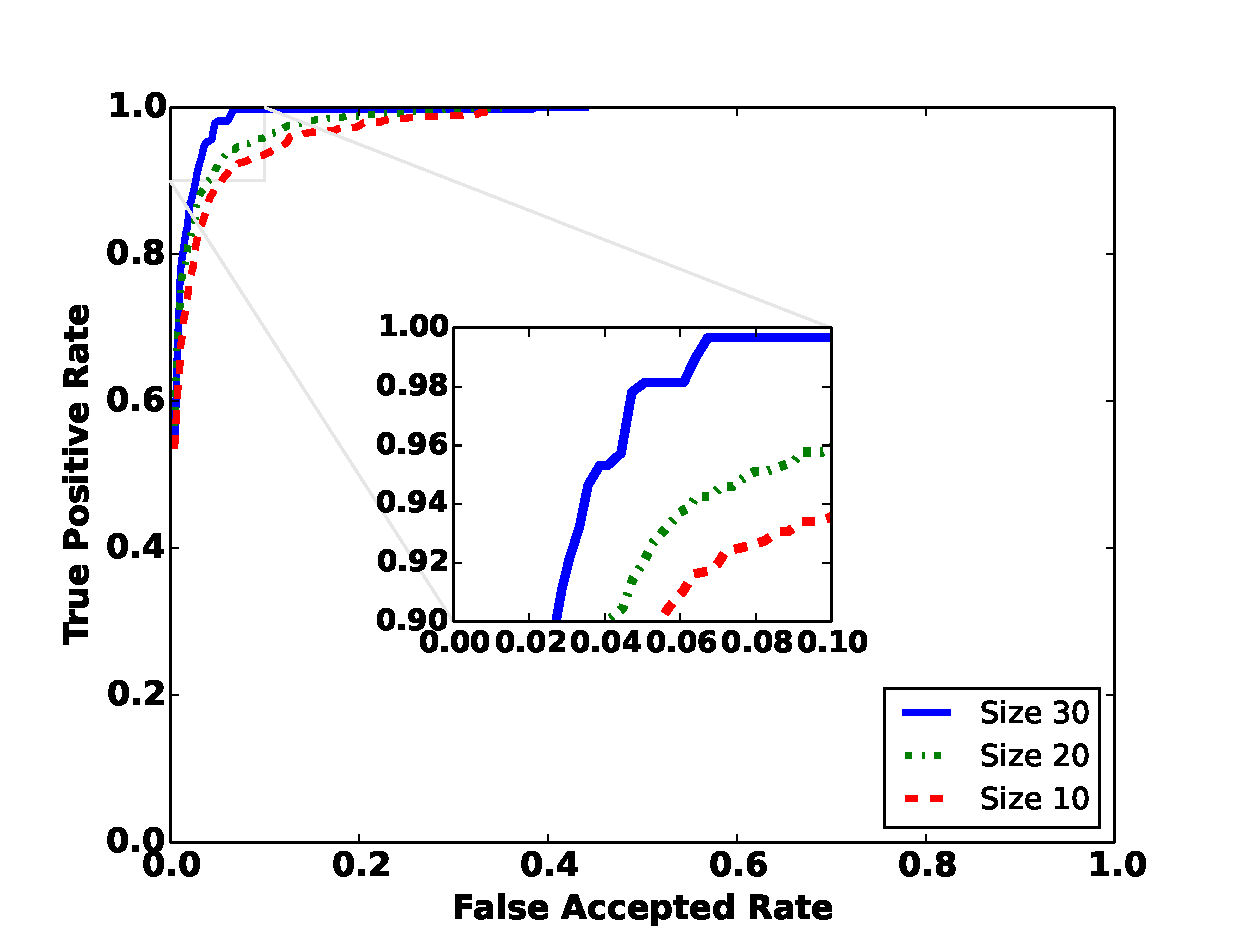
\includegraphics [width=\columnwidth]{figure/roc_diff_size.eps}
\caption{The impact of training dataset size: 10, 20, and 30 samples. In this set of results, we varied the value of $n$ from 0.0 to 10.0 with an increment of 0.1, resulting in 100 data points in each case. We then plotted the TPR (y-axis) and FAR (x-axis) for each data point. The results show that having 30 samples can considerably outperform than having fewer samples. As a result, in the remaining of the study, we will choose to have 30 samples.}
%The variable here is $n$. Each (TPR, FAR) data point in the curve corresponds to a different value of $n$}
\label{fig:roc_diff_size}
\end{figure}

%\begin{figure}[t]
%\centering
%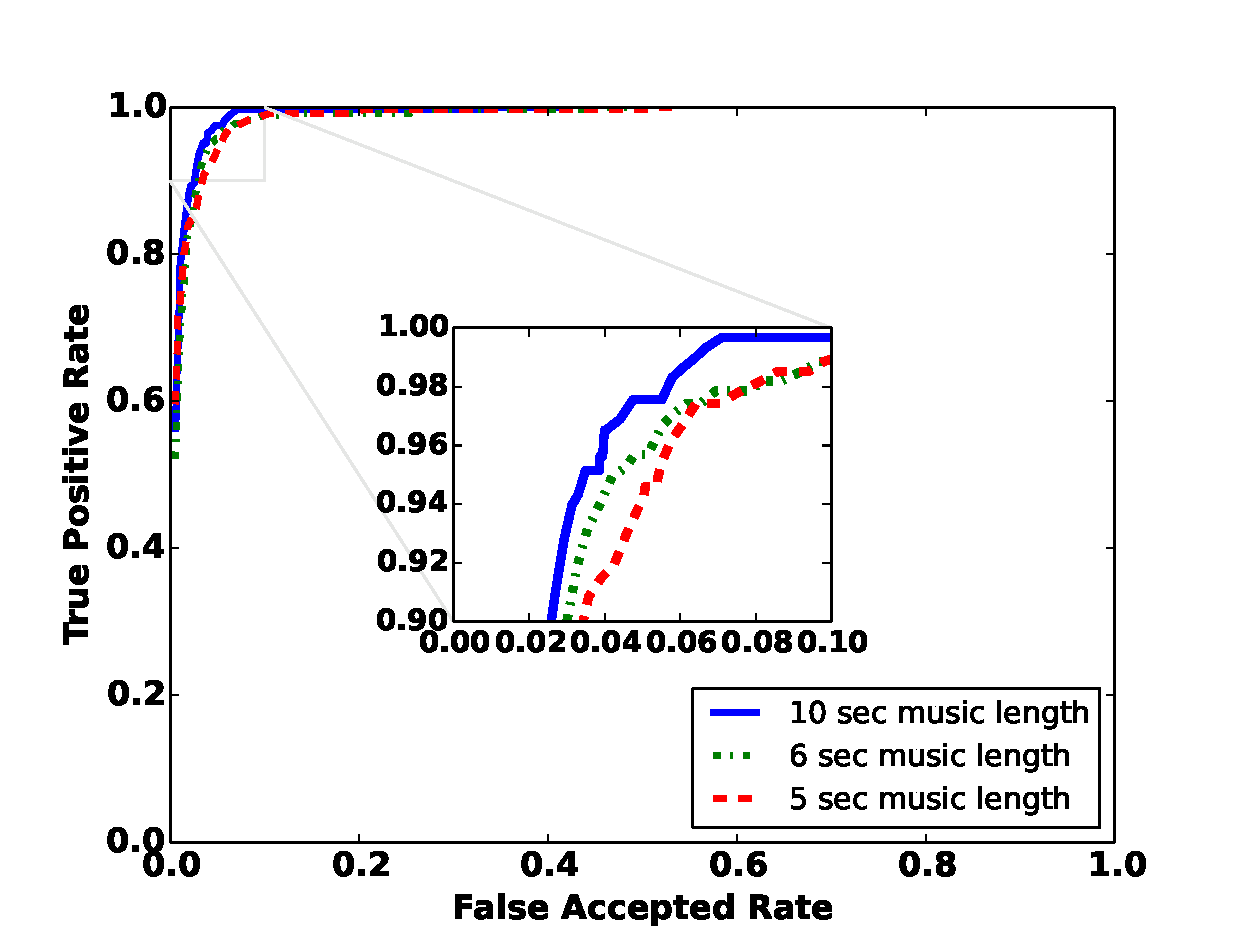
\includegraphics [width=\columnwidth]{figure/top3_roc.eps}
%\caption{Evaluation of impact of music cue duration on TPR and FAR in Top-3
%voting scheme ($K = 3$). A 10 sec music snapshot is trimmed into music cues of
%10 sec, 6 sec and 5 sec correspondingly.The variable here is $n$. Each (TPR, FAR) data point in the curve corresponds to a different value of $n$}
%\label{fig:roc-top3}
%\end{figure}

\begin{figure}[t]
\centering
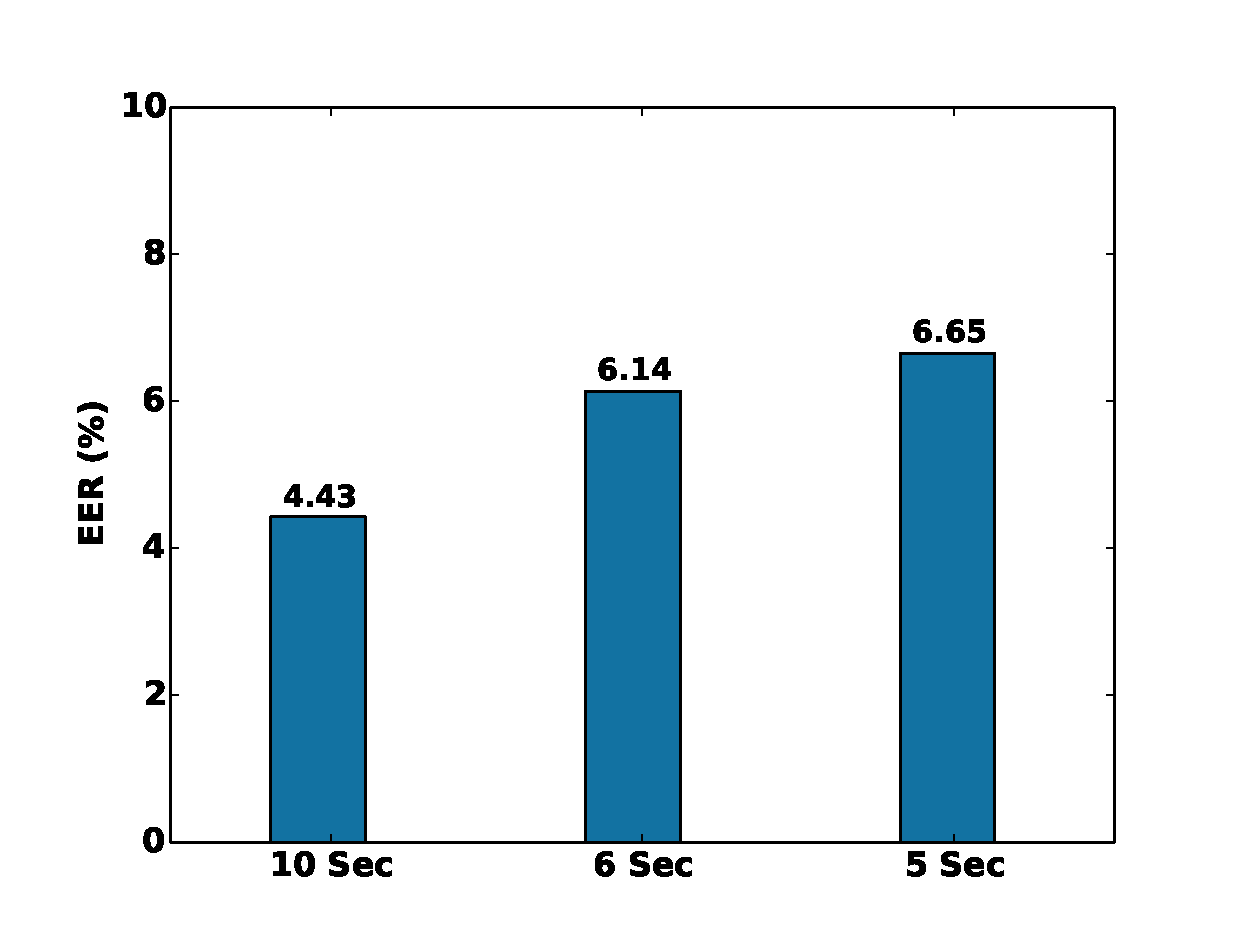
\includegraphics [width=\columnwidth]{figure/exp2_eer_vary_length.eps}
\caption{The EER of \systemname~when users choose different music cue lengths (10 sec, 6 sec and 5
sec) with a fixed n value of 2.7. We point out that ***}
\label{fig:eer-length}
\end{figure}




\subsection{Authentication Accuracy of \systemname}

\subsubsection{Participants}
We had a total of 30 volunteer participants for this experiment, including a total of 19 males and 11 females.
The average age of the participants was 29.7 years with a standard deviation
of 9.81 years. The youngest participant was 23 years old while the eldest was
54 years old.

\subsubsection{Procedure}
Our first experiment setup aimed at emulating the typical usage scenario
of \systemname~for authentication, where a user conducts head-movements in
response to a music cue played on the Google Glass device during a login
attempt.
%One of the participants executing the experiment trial wearing the
%Google Glass. %Figure~\ref{fig:setup} shows our experiment setup.
In this experiment, all participants were asked to wear a Google Glass
device. Participants who originally wore spectacles were asked to remove their
spectacles before conducting the experiment.
The trials were conducted in an academic environment and overseen by one of
our team members.
The Google Glass ran our data-collection app that played a piece of
music (music cue) for a specific duration, and recorded the accelerometer
sensor readings. We conducted these trials for three duration values: 5s,
6s and 10s. %As we will show further, the accuracy of the system can
%significantly improve with the duration of the music cue; longer the duration
%better is the accuracy.
The sensor readings were recorded into a text file that was stored
in the Glass's memory and later transported to a PC for offline processing
through a Python script. The experiment was conducted in a well-lit indoor
academic laboratory environment.

During the course of a data collection session, the participants were allowed to take a
break or withdraw from data collection if they felt uncomfortable at any
point; for example, feeling
dizzy after head-movement for a period of time, not being able to see clearly
if near-sighted, etcetera. The conductor also allowed the user to take a break
of about one minute after each trial.
Each trial lasted for the duration of the music cue played on the Glass, and
a total of 40 such trials were conducted for each of the 30 subjects.
The entire data collection effort lasted over a duration of 60 days, of which 15
subjects conducted their trials in a single sitting over a period of two
hours, while the rest of the trails were spread over 3 days on an average per
subject.
%while, half of the trials of the rest 10 subjects were spread over 2 days.
The experiment yielded three sets of data traces that each correspond to
the three music cue durations we selected.

\subsubsection{Metrics}
We evaluate the accuracy of \systemname~using metrics that are commonly used
in evaluating authentication systems, namely,
true positive rate TPR (percentage of true test samples that are
correctly accepted), false acceptance rate FAR (percentage of false test samples that are
mistakenly accepted), and false rejection rate TRR (percentage of true test
samples that are mistakenly rejected). These three metrics are, however, largely dependent on the choice of thresholding values in the system design --
a strict threshold in the classifier can lead to high TRR, while
overly relaxing the same can lead to a high FAR. Hence, in order to report the threshold-independent performance, we consider equal error rate EER (percentage of errors when $FAR = TRR$), that
balances FAR and TRR.
%%and balanced accuracy BAC, where BAC = 1 - (FAR+FRR)/2.
%%We present the accuracy results through the receiver operating
%%characteristics (ROC) curves, TPR versus FAR, as shown in Figures~\ref{}
%%and~\ref{}.
%Figures~\ref{fig:roc-top1}, \ref{fig:roc-top3} and \ref{fig:eer-length} report
%the accuracy
%of \systemname~through the metrics stated above.
%%Figures~\ref{fig:roc-curves} (a)-(c) report the accuracy of
%%\systemname~through the metrics stated above.

%In general, we observe that even with a 5s music cue, \systemname~can achieve a TPR of ***\% at FAR of ***\% and EER of ***\% (when we have $K$=***, *** out of 40 trials from each user being used for training with  thresholding parameter value $n = 2.7$ with DTW). If users do not mind a cue duration of 10s,

%After evaluating the above metrics under various scenarios, the highlight is that \emph{our TPR can be as high as 95.1\% at FAR of 3.5\% and EER of 3.97\%} (when we have $K = 3$, and 30 (out of 40) trials from each user being used for training with a thresholding parameter value $n = 2.7$ with DTW). Next we discuss in more detail how the authentication accuracy results are impacted by various design parameters.

\subsubsection{Tuning Important System Parameters}
Before presenting final authentication accuracy results, we first study how \systemname's performance is impacted by several important system parameters -- the choice of distance computing algorithm, $K$ value, and training dataset size -- and present the results  in Figures~\ref{fig:roc_dtw_cos_cor}-~\ref{fig:roc_diff_size}, respectively. Based upon these results, we tune the parameter values to balance the tradeoff between authentication accuracy and computing overhead. For each parameter study, we varied the value of $n$ from 0.0 to 10.0 with an increment of 0.1, and had a total of 100 data points. We then plotted the TPR  on y-axis and FAR on x-axis for each data point,  resulting curves referred to as Receiver Operating Characteristics (ROC) curves. ROC curves are usually used to describe the performance of an authentication system by varying the threshold~\cite{hanley1982meaning}.  ***YZ: varying the threshold? Unclear to me. *** In this setting, between two ROC curves on the same figure, the one closer to the upper left corner of the figure yields fares better than the other one.

Firstly, Figure~\ref{fig:roc_dtw_cos_cor} compares the performance of three distance computing algorithms: DTW, Cosine Distance, and Correlation, assuming $K=1$, music cue duration of 10s, and training dataset size of 30 samples.  Among these three algorithms, DTW fares much better than the other two: its EER is 14.29\% smaller than that of Cosine Distance, and 20.51\% smaller than that of Correlation. This is as expected because DTW is designed to match the waveform of two signals~\cite{dtw} and thus outputs more accurate distance score. As a result, in the remaining of this study, we will use DTW for the evaluation.


Secondly, Figure~\ref{fig:roc_k_value} compares the performance of two $K$ values: $K$=1 and $K$=3, assuming DTW distance, music cue duration of 10s, and training dataset size of 30 samples.  Recall that the classification algorithm in ~\systemname~generates a classification result (YES or NO) by voting among individual results each generated by the top-K samples in the true set. Hence, we expect that considering top 3 samples will be better than only considering the top 1 sample, as confirmed by the results shown in Figure~\ref{fig:roc_k_value}. However, we observe the improvement is very marginal: the EER when $K=3$ is only 0.5\% smaller than the EER when $K=1$. On the other hand, having $K=3$ incurs three times as much computing as having $K=1$. As a result, in the remaining of this study, we will use $K=1$ for the evaluation.

Thirdly, Figure~\ref{fig:roc_diff_size} compares the performance of three training dataset sizes: 10, 20, and 30 samples, assuming DTW distance, $K=1$, and music cue duration of 10s. We observe that the EER when $size=30$ is 1.79\% better than the EER when $size=20$ and 3.17\% smaller than that when $size=10$. As a result, in the remaining of this study, we will use $size=30$ for the evaluation.

%\paragraph{Impact of Training Dataset Size}
%%The accuracy of detecting and matching the head-movements to the user depend
%%upon the music cue duration, value of $K$, and number of samples used for
%%training.

%***YZ: we need to rewrite this section. In this section, we need to focus on how much improvement we have when we increase the data set size. Also, I think we are using way too many metrics. ***
%Recalling from Section~\ref{sec:design}, the input to the training phase
%is a set of temporal signals (samples with duration equal to the music cue
%duration), each corresponding to one trial of the head-movements from the
%user. Our evaluations so far considered a training set consisting of 30 samples.
%***I feel we have too many different metrics. It is confusing.*** In Figure~\ref{fig:eer-size}, we report the EER in \systemname~for three
%different training data set sizes; 10,20 and 30 samples.
%We can observe from Figure~\ref{fig:eer-size} that the EER holds an inverse
%relationship with the training set size. A larger training set minimizes the
%variance in mean and standard deviation computations, as the errors in their
%inconsistency are reduced by averaging the mean and standard deviation
%estimates over a larger set of data.
%On the other hand, a larger training set also implies a longer execution time
%of the training phase.
%However, in our system design, we posit that the training phase can be
%conducted
%offline on a more compute efficient device (smartphone, PC or server) and that
%the wearable device can pre-fetch the trained data (for example, an XML file),
%prior-to or during data collection phase, through a wireless link.

%are giving promising results for the response time sequence, hence we will evaluate these three algorithms in our end-to-end system. Also due to DTW is relatively more computing-intensive than the other two algorithm, we would like to see whether DTW  is worth of computing resource. In this experiment, we vary thresholding parameter value $n$ and fix the other parameters: 10 sec duration, $K = 1$, and  training data $size = 30$. We can observe from the ROC
%(receiver operating characteristic) curves in Figure~\ref{fig:roc_dtw_cos_cor} that DTW gives the best result among three algorithms, since its curve is the closest to the upper left corner. Our system preserves all characteristics of the data, which includes the response time to the music beat and the 3-axis accelerometer data. In terms of ~\cite{DTW}.

%\paragraph{Impact of $K$ value}
% We observe from the ROC curves in Figure~\ref{fig:roc-top1} and \ref{fig:roc-top3} that
%for both, $K=1$ and $K=3$, the TPR is close to 95\% while the FAR is slightly
%above 3\% for the 10 sec music duration. For $K = 1$ the FAR increases to
%about 7\% for the 5 sec and 6 sec cases, however, for $K = 3$ the FAR
%decreases to about 3\% and 4\%, respectively.
%We observe a similar trend with the EER as shown in
%Figure\ref{fig:eer-length}, where improvements of 0.5 - 1 \%
%can be achieved by choosing $K = 3$ over $K = 1$. ***YZ: if the improvement is less than 1\%, then K=1 is sufficient. Then for the music cue, please just use K=1***
%This indicates that the accuracy in \systemname~can improve with a larger
%value of $K$. However, the improvement in accuracy through redundancy in the
%training set trades off with the increased execution time as the
%matching requires at least $K - 1$  extra DTW computations as opposed to only
%1 for a top-1 scheme. As we will show ahead, DTW computations incur heavy CPU
%budget on the wearable device.
%***YZ: I will re-write this paragraph after you reorganize the results ***
Finally, we note that in Section~\ref{subsec:app}, we have implemented a Headbanger app for Google Glass, and measured the computing latency of the app using the chosen parameter values. We show that the resulting computing latencies are very reasonable.


\subsubsection{Authentication Accuracy Results}
%We measure the DTW computation on Google Glass to be the most
%computationally expensive operation of all the software modules in
%\systemname.
%\paragraph{Impact of music cue duration}

%***YZ: I need to rewrite this paragraph. The tone needs to be changed. What is the improvement? ***

After tuning system parameters, we next calculate the EER of~\systemname~when users choose different music cue durations and present the results in Figure~\ref{fig:eer-length}. As soon as a user starts the authentication procedure, how long the user must wait before she receives the authentication result is an important quality-of-service metric, which we refer to as \emph{authentication latency}.  Authentication latency consists of two parts: data input latency and computing latency, where the former is the time a user spends on listening to the music cue and making head movements while the latter is the time \systemname~spends on computing the authentication result. Between these two parts, data input latency is the bottleneck as the computing latency can be easily reduced (by better algorithms and/or faster hardware) and/or hidden (by pipelining computing with data collection). Unfortunately, data input latency is hard to be reduced or hidden by the improvement in software or hardware. Recognizing that different users can tolerate different latencies and desire different levels of authentication accuracies, \systemname~allows the users to choose the music cue duration (which has the same length as the data input latency).

From Figure~\ref{fig:eer-length}, we observe that the EER of \systemname is as low as 6.65\% with a 5-second music cue, and 4.43\% with a 10-second music cue. We take the viewpoint that this accuracy is rather sufficient for personal wearable devices that are not used in very hostile environments.
%
%In general, we observe from the results that the FAR can
%be decreased by increasing the music cue duration.
%We can observe (from Figures~\ref{fig:roc-top1}, \ref{fig:roc-top3} and
%\ref{fig:eer-length}) that the improvement is less significant when the music
%cue duration is increased from 5 sec to 6 sec, however, the improvement is
%more
%significant when the music cue duration is increased to 10 sec.
%In \systemname~the data collection phase for the authentication system
%(sampling accelerometer sensor readings) is executed in parallel with the
%music cue. The data processing phase involving the filtering, classification
%and matching is executed only at the end of the music cue and in the same
%order.
%Hence, execution time of the app will be independent of this duration.
Finally, we note that, the data input duration of 5-10 sec for authentication is on par with those
of PIN-based and pattern-based system~\cite{von2013patterns}, where the former takes 1.5 sec and the later takes 3.1 sec on average. ***YZ: 5-10 seconds are much larger than 1.5/3.1 seconds!!***
%We also note that, since the authentication process is initiated only at the
%end of the music cue, execution time of the app will be independent
%of this duration.

%\begin{figure}[t]
%\centering
%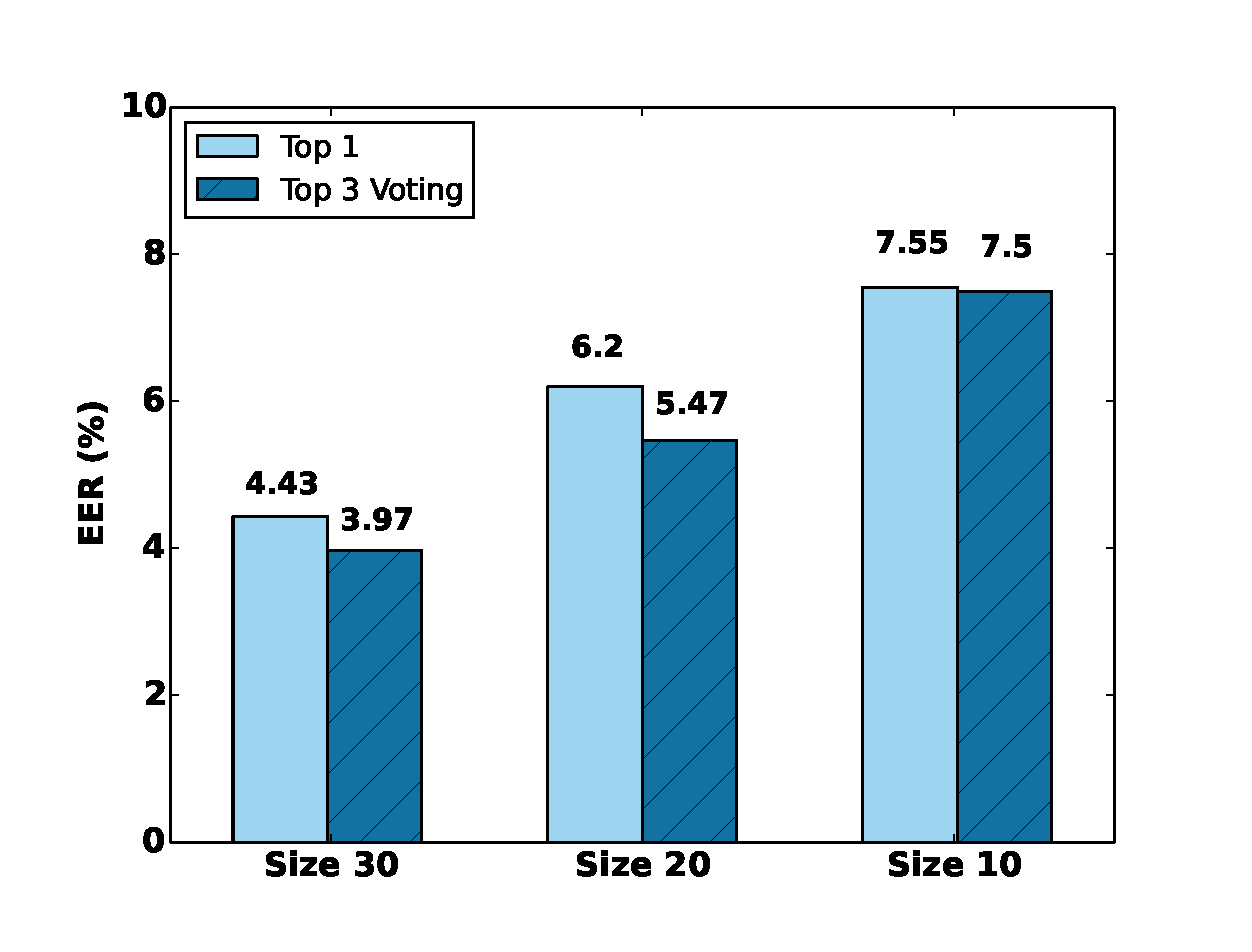
\includegraphics [width=\columnwidth]{figure/exp2_vary_size.eps}
%\caption{Comparison of EER for different training sample sizes (30, 20 and 10)
%with fixed n value of 2.7}
%\label{fig:eer-size}
%\end{figure}





%\paragraph{Impact of Sampling Rate}
%***YZ: this can be removed ***
%Due to DTW is resource-consuming, one direct way to reduce the workload of our algorithm is to decrease the sampling rate of the accelarometer and remain the sampling time. Based on Nyquist–Shannon sampling theorem, since the high cut of our filter is 10 Hz, the minimum sampling rate should be 20 Hz. Also, the highest sampling rate and the default sampling rate of our platform are 200 Hz and 50 Hz accordingly. Thus, we choose these three value to evaluate the impact of sampling rate.  In Figure~\ref{fig:roc_dtw_diff_freq}, we observe that 200 Hz provides the best performance among three value, while 50 Hz and 20 Hz are giving closed results. The EER of 20 Hz is **, comparing with  ** of that of 200 Hz. Since the decrement of EER is insignificant and we can achieve 10 times speedup in DTW computing,  20 Hz will be a ideal value of system implementation.
\begin{figure}
\centering
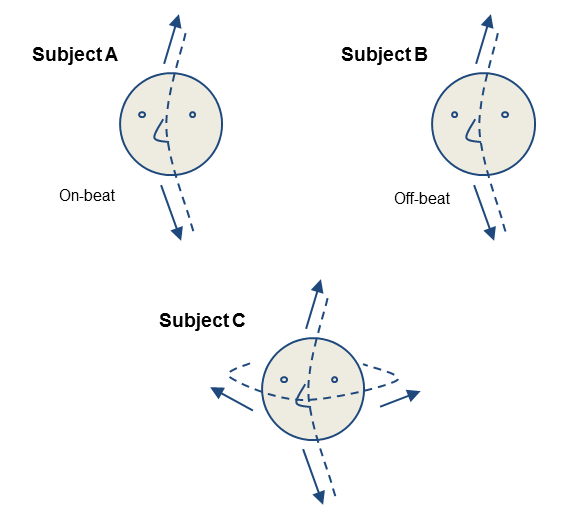
\includegraphics[width = \columnwidth]{figure/imitation_subject_movement.png}
\caption{\label{fig:imitation_movement} Pictorial description of how the mimicked subjects move.}
\end{figure}


\subsection{Authentication Robustness of \systemname} After evaluating authentication accuracy for \systemname, we next study its robustness against imitation. For this purpose, we asked a number of subjects (imitators) to imitate simple nodding patterns from three subjects (imitatees) after watching the imitatee's video for as long as they desire, and calculated their chances of successful imitation - i.e., the imitator is mistakenly accepted by \systemname. We note that nodding is the simplest head-movement pattern and easiest to imitate; hence, the results presented here represent the \emph{lower bound} robustness that \systemname~offers. In reality, users are more likely to employ more sophisticated head-movement patterns, which will be much harder to imitate.

\subsubsection{Participants}
We had a total of 37 volunteer participants, including 31 males and 6 females. The average age of the participants was 25.6 years with a standard deviation
of 6.6 years. The youngest participant was 22 years old while the eldest was 49 years old.

\subsubsection{Procedure}
Our second experiment aimed at emulating a practical imitation attack scenario. In this experiment, three imitatees recorded video when they were nodding with a music cue. Note that the music is usually played via a bone conduction speaker or an earplug, and that it is difficult to use a camcorder to capture the music sound in a noisy environment. To address this concern, during recording, we set the speaker volume to maximum and conducted the recording in a quiet laboratory environment.

We divided the imitators into three group, and asked each group to imitated one imitatee. In each session (consisting of 30 trials), the imitator could watch the video for as long as they wish. Our system provided a feedback after each trial so that the imitators could adjust their nodding pattern if they wanted. After the imitator had 30 trials,
we ended the session no matter whether the imitator had succeeded or not. In each session, we noted the total number of successes the imitator had as well as the number of trail before the first successful imitation. %This experiment was conducted in quite space on campus. We will now discuss our evaluation results for both experiments in detail.

\subsubsection{Results}
Each of the three imitatees performed simple nodding in this experiment; though simple, their nodding patterns have varying complexity. As shown in Figure~\ref{fig:imitation_movement}, Imitatee $A$ moved his head vertically, each nodding on a music beat, with no noticeable horizontal movement; imitatee $B$ also only moved his head in the vertical direction, but there was always a delay between his nodding and the corresponding music beat; imitatee $C$ combined slight shaking along with nodding, and closely followed music beats. Among these three imitatees, $A$ is the easiest, while the other two are slightly more complex.

Table~\ref{tab:imitation} summarizes the results. Here, we use FAR to denote the successful imitation rate because a successful imitation is also a false acceptance. The overall FAR of the experiment is 7.54\%, while the individual FARs for the three imitatees are 15.83\%, 2.77\% and 2.72\% accordingly.  Since imitatee $A$ had the easiest nodding pattern, 6 out of 10 subjects could succeed at least once during their 30 trials, while for imitatees $B$ and $C$, the numbers are  3 out of 13 and 3 of 12, respectively. These results are promising: when a user employs slightly more complex head-movement patterns, it becomes much harder for others to imitate. 



\begin{table}[b]
\centering
\begin{tabular}{|l|c|c|c|c|}\hline
                               & No. &  No. &  Average No. of  &  \\
Imitatee & of & of & Trials Before & FAR (\%) \\
& Imitators & Successful Imitators & First Successful Login & \\\hline

A                   & 12                                 & 7                                                                     & 10.33                                                                                               & 15.83                        \\ \hline

B                   & 13                                 & 3                                                                     & 14.33                                                                                               & 2.77                         \\ \hline

C                   & 12                                 & 3                                                                     & 17.67                                                                                               & 2.72                          \\ \hline\hline

Overall & 38                                 & 13                                                                    & 13.17                                                                                                    & 6.94                         \\ \hline
\end{tabular}

\caption{\label{tab:imitation} The imitation results show that as head-movement patterns become more complex, it becomes much harder to imitate. }

\end{table}



\subsection{Headbanger Google Glass App Implementation}\label{subsec:app}

\begin{figure}[t]
\centering
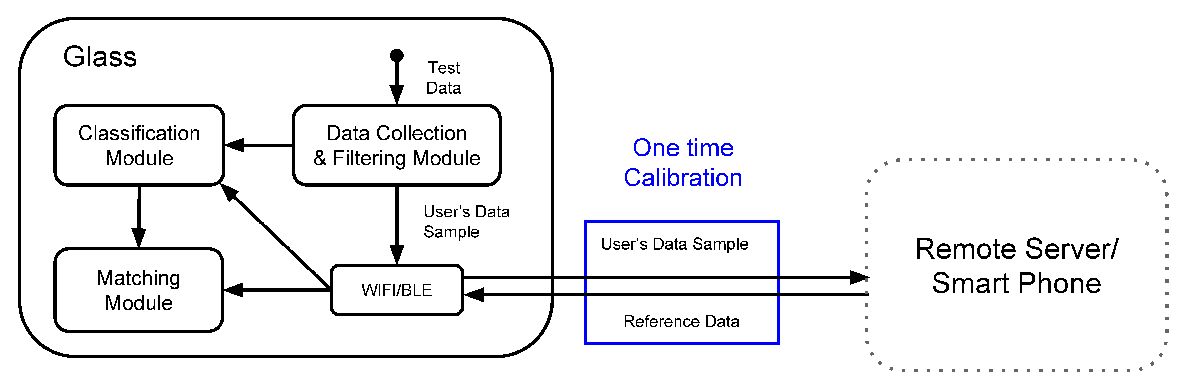
\includegraphics [width=\columnwidth]{figure/software_arch.eps}
\caption{Software modules of \systemname~implementation}
\vspace{25 pt}
\label{fig:glass-softwarearch}
\end{figure}

In the second phase of evaluation, we implemented \systemname~on Google glass, positioning it as an
authentication application (app).
Figure~\ref{fig:glass-softwarearch} shows the main software modules in the
app. Upon initiation by the user, the app plays a music cue for a user-specified
duration. The user conducts head-movements in synchrony with the music cue
while the app records the accelerometer data in parallel. At the end of the
music cue duration the app enters the data processing phase where the
sensor readings are input to the \systemname's software modules for
processing. %The processing stage includes the filtering of the accelerometer
%sensor values, classification and feature extraction using DTW, and threshold
%based matching of the generated features with those from training set.
%%\systemname extracts the head-movement features through
%%the thresholding process discussed in section~\ref{sec:design}, and compare
%%with the feature templates generated from the training phase.
Upon completion of data processing, the app responds with a YES or NO textual
output on the Google Glass screen. The training phase is conducted offline on a PC, and %prior to live-testing off the application.
%The training phase 
%which involves collecting 30 samples of the
%head-movement accelerometer readings, generating the features, and saving them
%into a local server (running on PC) as an XML file, with appropriate indexing.
%Upon app initiation on Glass, the trained features are pre-fetched from
%the server through a wireless connection. 
we ensure that the training set
is readily available during the authentication process. %thus eliminating the
%additional processing time required for the training phase.
%Conducting online training, particularly that involves DTW computations, is
%very compute intensive on a resource constrained devices such as Glass.
%One possible solution would be for the Glass to offload the
%training phase computation to a local server machine.
%We reserve such considerations for future implementations.

%Among all the software modules, the ``training set construction model'' is
%the most computing-intensive, and as a result, we executed the model on the
%bluetooth-paired smartphone. The rest of the modules are implemented and
%executed on the glass.
%In our on-glass app, the classification module runs the
%thresholding-based classification.
\subsubsection{Data Processing Latency}

\begin{table}[b]
\centering
\begin{tabular}{|ccclc|}
\hline
\multicolumn{1}{|c|}{\multirow{2}{*}{\begin{tabular}[c]{@{}c@{}}music  cue \\
duration (s)\end{tabular}}} &
\multicolumn{1}{c|}{\multirow{2}{*}{\begin{tabular}[c]{@{}c@{}} data processing latency (s)\end{tabular}}} & \multicolumn{3}{c|}{time breakdown (\%)}
\\ \cline{3-5}
\multicolumn{1}{|c|}{}
                             &
\multicolumn{1}{c|}{}
                              &
 Filtering & \multicolumn{1}{c}{DTW} & Thresholding   \\
 \hline\hline
10
                             &
1.93
                              &
 0.50      & 99.50                   & \textless0.01  \\
6
                             &
1.15
                              &
 0.64      & 99.36                   & \textless0.01  \\
5
                             &
0.88
                              &
 0.81      & 99.19                   & \textless0.01 \\ \hline
\end{tabular}
\caption{\label{tab:glass} Measured response time of \systemname~app implementation on Google
Glass with different music cue durations and for $K = 1$. The response time
reported here is an average over 20 trials.}

\end{table}

In Table~\ref{tab:glass} we report the measured average processing latency
of the \systemname~app for music cue durations
of 5, 6 and 10 seconds. %We conducted the benchmark execution-time profiling of
%\systemname~on Glass in a controlled indoor laboratory setting with no
%mobility. We define response time as the time elapsed between music cue
%completion to
%the display of authentication response (YES/NO text) on the Glass screen.
The processing latency is within 2 seconds for a 10-second data input, and is less than 1 second (0.88s) for a 5-second input.  
%We feel that a response time of 2-5 sec for a local authentication solution in
%Google Glass is comparable to that of prior-art that comes close to our
%solution~\cite{von2013patterns,egelman2014you}.
%It is important to note that authentication solutions that execute
%locally on head-worn wearable devices, especially on a heavily resource
%constrained device like Glass, are still not mature. However, the hope is that
%such solutions will possibly catch up to speed in the near future and that our
%approach is advancing one step in that direction.
We also report the total latency breakdown for different software modules, and find that DTW computation is the main bottleneck. In our implementation, we used Fast DTW~\cite{salvador2007toward} which provides about 2x speed-up in DTW computation without compromising the authentication accuracy.
%We can observe from Table~\ref{tab:glass} that the DTW computation
%dramatically compute intensive than the other processes.

As we discussed earlier, the processing latency can be further reduced, and it could be partially hidden if we pipeline the data processing and data input. As a result, we believe that it is realistic to run the \systemname~app on devices that have comparable computing capabilities as the Google Glass.
%It is important to note that our current implementation uses a faster
%version of the DTW algorithm called Fast DTW~\cite{salvador2007toward},
%providing about 2x speed-up in DTW computation.
%We believe that the response time can be reduced
%further through strategic methods such as, further optimizations in the Fast
%DTW algorithm or pipelining the app execution along with data collection.
%A specific strategy for reducing response time for rejected attempts can be
%that, after a short duration, before the entire music cue is played, if it is
%found that a user's movement does not match the signature of the claimed user
%with a sufficient pre-determined confidence level, then the on-site
%classification may be terminated instead of waiting for the entire duration to
%yield the rejection.
%Another example, may include cyber-foraging strategies to offload heavy
%computation tasks, such as online training and classification, to the user's
%Bluetooth paired smartphone or a nearby cloudlet~\cite{ha2014towards}.

 